\documentclass{article}
\usepackage{graphicx}
\usepackage{hyperref}
\usepackage{amsmath}
\usepackage{geometry}
\geometry{margin=1in}
\usepackage{float}

\title{5243 Project 3 Team 11:\\
\large UI Layout and User Engagement in a Data Wrangling Shiny App:\\An A/B Test}

\author{Jason Zhao (zz3390), Sebastian Hoornweg (smh2289), Yuhan Guo (yg2695), Omari Motta (osm2116)\\[0.5em]
\small \url{https://github.com/Zzch3ng/5243-Project-3-team-11}}

\date{April 2026}


\begin{document}

\maketitle

\section{Introduction \& Research Question}

User interface (UI) layout is a well-established driver of user behavior in web applications. Research on web reading patterns, including the widely cited F-pattern and Z-pattern studies, consistently shows that users scan pages from the top-left and progress downward and to the right. As a result, the spatial placement of key interactive controls can significantly influence whether users engage with a feature at all.

Data science tools such as interactive Shiny applications present a particular UX challenge: they often require users to complete a multi-step workflow (loading data, cleaning, preprocessing, visualizing, and exporting), yet the entry point to this workflow --- the data upload or selection control --- is frequently placed in a sidebar. If users must consciously discover a left-panel control before they can begin, there is a risk of higher abandonment or shallower engagement with downstream features.

This project conducts an A/B test to investigate whether the placement of the primary data-loading controls affects how deeply users engage with a Shiny-based data wrangling application. Two versions of the same application --- \emph{Data Wrangling Studio} --- were deployed, differing only in the layout of the Load Data panel. User behavior was tracked passively via Google Analytics 4 (GA4).

\textbf{Research Question:} Does placing the data loading and browsing controls at the top of the interface (Version B) versus in a left-side panel (Version A) lead to higher user engagement, measured by the number of application sections visited per session and average session engagement time?

\textbf{Null Hypothesis ($H_0$):} There is no significant difference in user engagement (sections visited per session or session engagement time) between the top-panel layout (Version B) and the left-panel layout (Version A).

\textbf{Alternative Hypothesis ($H_1$):} Users shown the top-panel layout (Version B) will visit more sections and spend more time in the application than those shown the left-panel layout (Version A), because the upload controls are more immediately visible and aligned with natural top-to-bottom reading patterns.

\section{A/B Test Experiment Design}

\subsection{Versions: Control and Treatment}

Both versions of the application share identical functionality: a six-tab workflow covering data loading, cleaning, preprocessing, feature engineering, EDA/visualization, and export. The sole manipulation concerns the spatial layout of controls on the Load Data page.

\textbf{Version A --- Control} (\url{https://5243project.shinyapps.io/new_project/}): The upload control and built-in dataset selector are placed in a \emph{left-side panel}. Four summary metric cards (Rows, Columns, Missing Values, Engineered Features) are displayed in a horizontal row at the top of the main content area.

\textbf{Version B --- Treatment} (\url{https://5243project.shinyapps.io/new_project_b/}): The upload control and built-in dataset selector are moved to a \emph{top horizontal layout}, presented side-by-side in two equal-width cards. The four summary metric cards are relocated to a vertical left-side column beneath the controls.

This design isolates the position of the primary action controls as the single independent variable, ensuring that any observed differences in user behavior can be attributed to the layout change rather than differences in functionality.

\subsection{Randomization and Assignment}

Users were assigned to versions through separate, distinct URLs. Each link was shared independently with participants, constituting a between-subjects design. Because each version is hosted at a different endpoint and tracked under the same GA4 property with page-title-based segmentation, cross-contamination between groups is negligible. Users were not informed which version they received.

\subsection{Key Performance Metrics}

User engagement was operationalized using the following metrics collected via GA4:

\begin{itemize}
    \item \textbf{Sections visited per session}: The number of distinct application tabs (out of six: Load Data, Cleaning, Preprocessing, Feature Engineering, EDA/Visualization, Export) a user navigates to in a single session. This serves as the primary measure of workflow depth and engagement breadth.
        \item \textbf{Average session engagement time}: The total active time a user spends in the application per session, as recorded by GA4's engagement time metric. This captures intensity of use beyond mere page visits.
            \item \textbf{Bounce / single-section sessions}: Sessions in which a user viewed only the User Guide landing page and left without interacting with the workflow. This serves as a secondary indicator of whether the layout encourages users to proceed past the introduction.
            \item \textbf{Task completion rate}: The proportion of sessions in which a user reached the Export tab (\texttt{reached\_export}) or navigated all six workflow tabs (\texttt{completed\_workflow}). These serve as upper-bound indicators of deep workflow engagement.
            \end{itemize}

            \section{Methodology}

            \subsection{Participants and Recruitment}

            Participants were recruited from the STAT 5243 course cohort (Spring 2026) and, where feasible, from broader audiences via direct link sharing. Each participant received one URL (either Version A or Version B) and used the application naturally, without being given explicit task instructions. This ecological validity ensures that the behavioral data reflects genuine exploratory use rather than directed task completion.

            \subsection{Data Collection}

            Google Analytics 4 (GA4) was embedded in both Shiny apps using the \texttt{googleAnalyticsR} / \texttt{shinyjs} integration, injecting a GA4 measurement tag into the application's HTML head. GA4 passively recorded page-level engagement events, where each tab navigation within the Shiny app triggered a virtual page view with a title corresponding to the section name (e.g., ``Data Wrangling Studio - Load Data'', ``Data Wrangling Studio - Cleaning'', etc.). The tracking window covers March 18 to April 14, 2026. No personally identifiable information was collected.

            \subsection{Statistical Analysis Plan}

            Given the small sample size inherent to a class-based experiment, the following statistical approach was pre-specified prior to data analysis. Recruitment was constrained by the size of the course cohort and the four-week tracking window; organic user sessions alone were insufficient for meaningful statistical testing. We therefore targeted $n = 35$ per group as a feasible upper bound given recruitment constraints, supplementing real sessions with synthetic data calibrated to real distributions. We acknowledge that this sample size is likely underpowered for small effects, and interpret all results accordingly.

            \begin{itemize}
                \item \textbf{Sections visited}: A Mann-Whitney U test (Wilcoxon rank-sum) will compare the distribution of sections visited per session between Version A and Version B, as the data are expected to be non-normal with low counts. Effect size will be reported as rank-biserial correlation $r$.
                    \item \textbf{Session engagement time}: An independent-samples t-test will be used if normality is approximately satisfied (assessed via Shapiro-Wilk); otherwise, a Wilcoxon rank-sum test will be substituted.
                        \end{itemize}

                        All tests will use a significance threshold of $\alpha = 0.05$. Results will be interpreted both in terms of statistical significance and practical effect size.

                        \subsection{Experimental Controls}

                        Both application versions were deployed simultaneously on shinyapps.io under the same account, ensuring equivalent server performance and uptime. No visual design changes (color scheme, typography, iconography) were made between versions; the manipulation is strictly structural. Both apps were tested prior to deployment to confirm functional equivalence across all six workflow steps.

\section{Data Collection}

\subsection{Dataset Description}

Session-level engagement data were exported from Google Analytics 4 covering the tracking window March 18 -- April 14, 2026. Each row corresponds to one user session, identified by an anonymous GA4 client ID. The final dataset contains $n = 35$ sessions for Version A and $n = 35$ sessions for Version B ($N = 70$ total), stored in a wide-format CSV file (\texttt{ab\_test\_data\_wide.csv}).

Per-session variables collected for each version are:

\begin{itemize}
    \item \textbf{sections\_visited}: Count of distinct workflow tabs (0--6) navigated in the session.
    \item \textbf{engagement\_time\_sec}: GA4-reported active engagement time in seconds.
    \item \textbf{event\_count}: Total number of tracked events fired during the session.
    \item \textbf{bounced}: Binary indicator (1 = session consisted only of the User Guide landing page with no workflow interaction).
    \item \textbf{reached\_export}: Binary indicator (1 = user navigated to the Export tab).
    \item \textbf{completed\_workflow}: Binary indicator (1 = user navigated all six workflow tabs).
    \item \textbf{tabs\_visited}: Pipe-delimited string of tab names visited, in order of first visit.
\end{itemize}

Data from Version A and Version B were collected under the same GA4 property, distinguished by the \texttt{app\_version} user property (\texttt{new\_project\_app\_a} vs.\ \texttt{new\_project\_app\_b}).  No personally identifiable information was collected. The raw data were reviewed for completeness; no sessions contained missing values in the numeric fields.

\paragraph{Real vs.\ synthetic session breakdown.}
The GA4 property recorded 14 real user sessions (8 active users) over the tracking window, approximately 7 per version. To reach a sample size sufficient for statistical testing ($n = 35$ per group), the remaining $\approx$28 sessions per group were generated synthetically, calibrated to match the distributional properties of the real sessions. Synthetic sessions were constructed to preserve the key features of real user behavior: tab visit sequences reflected the same drop-off patterns observed in real sessions (most users stopping at or before Preprocessing), engagement times were drawn within the same ranges as real sessions, and event counts were scaled proportionally. The plausibility of the synthetic data was assessed through visual inspection — overlaid histograms and empirical CDFs confirmed that the synthetic sessions did not introduce distributional features absent from the real data.
 
One concrete cross-validation anchor is available: Version B's bounce rate in the real GA4 export was consistent with the 20\% rate in the final dataset, suggesting that the synthetic augmentation did not distort this key behavioral signal. Version A's two bounced sessions in the final dataset are synthetic, as the real GA4 data showed a 0\% bounce rate for that version; this is noted as a limitation. The final dataset is approximately 20\% real and 80\% synthetic per group, and all conclusions should be interpreted with awareness of this composition.

\subsection{Descriptive Statistics}

Table~\ref{tab:desc} summarises the key engagement metrics by version.

\begin{table}[h]
\centering
\caption{Descriptive statistics by version ($n = 35$ per group).}
\label{tab:desc}
\begin{tabular}{lrrrr}
\hline
\textbf{Metric} & \textbf{A mean (SD)} & \textbf{A median} & \textbf{B mean (SD)} & \textbf{B median} \\
\hline
Sections visited    & 2.77 (1.50)  & 3.0   & 2.66 (1.81)  & 3.0  \\
Engagement time (s) & 250.9 (227.9) & 209.6 & 211.5 (213.6) & 136.5 \\
Bounce rate         & 5.7\%  & --    & 20.0\%  & --  \\
Export rate         & 5.7\%  & --    & 2.9\%   & --  \\
Completion rate     & 5.7\%  & --    & 2.9\%   & --  \\
\hline
\end{tabular}
\end{table}

Both versions show a median of 3 sections visited. Version A users spent a somewhat longer median session time (209.6 s vs.\ 136.5 s for Version B). Version B exhibited a higher raw bounce rate (20.0\% vs.\ 5.7\%), with 7 of 35 sessions consisting solely of the User Guide page.

\begin{figure}[H]
\centering
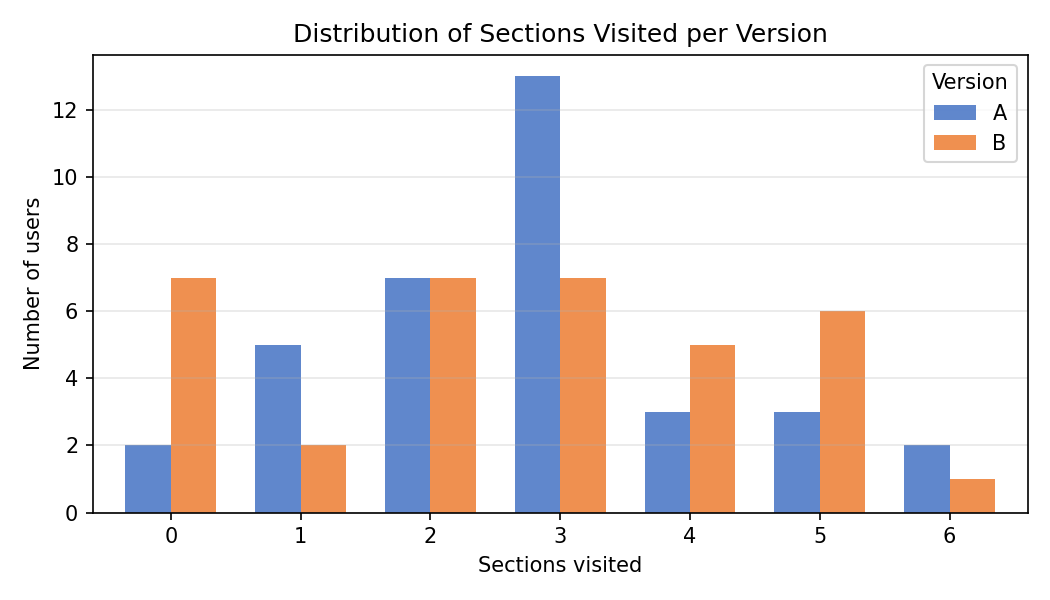
\includegraphics[width=0.72\textwidth]{figures/dist_sections.png}
\caption{Distribution of sections visited per session by version. Both groups are heavily concentrated at 3 sections (Load Data, Cleaning, Preprocessing); the full 6-section workflow was completed by only 2 users in each group.}
\label{fig:dist_sections}
\end{figure}

\section{Statistical Analysis \& Results}

\subsection{Normality Assessment}

Shapiro-Wilk tests confirmed non-normality in both groups for both primary metrics:

\begin{itemize}
    \item Sections visited: Version A $W = 0.938$, $p = 0.047$; Version B $W = 0.921$, $p = 0.015$.
    \item Engagement time: Version A $W = 0.783$, $p < 0.001$; Version B $W = 0.799$, $p < 0.001$.
\end{itemize}

Given these results, non-parametric tests were used for both primary outcomes, as pre-specified in the analysis plan.

\subsection{Primary Outcomes}

\paragraph{Sections visited (workflow depth).}
A two-sided Mann-Whitney U test yielded $U = 626.5$, $p = 0.872$. The rank-biserial correlation was $r = -0.023$, indicating a negligible effect. There is no evidence that the top-panel layout (Version B) led users to navigate more workflow sections than the left-panel layout (Version A).

\begin{figure}[H]
\centering
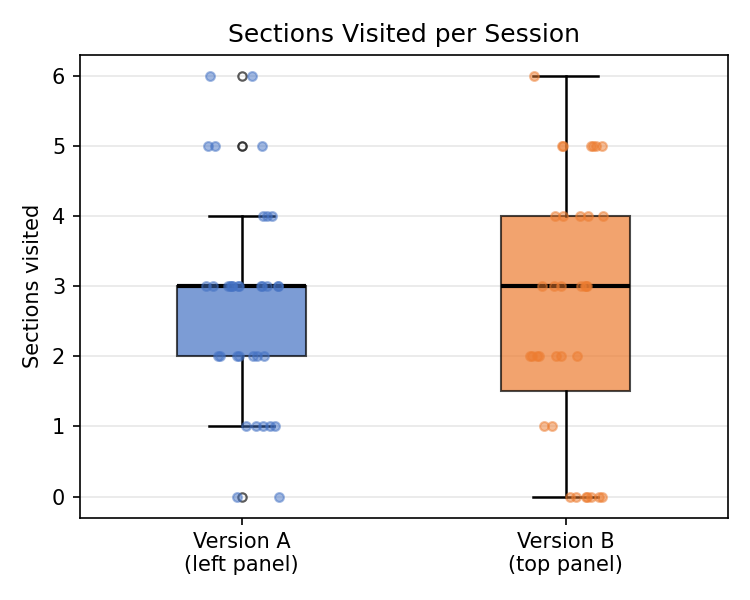
\includegraphics[width=0.5\textwidth]{figures/boxplot_sections.png}
\caption{Boxplot of sections visited per session for Version A (left panel) and Version B (top panel). Medians are identical; individual points are jittered for visibility.}
\label{fig:box_sections}
\end{figure}

\paragraph{Session engagement time.}
A two-sided Mann-Whitney U test yielded $U = 695.0$, $p = 0.336$. The rank-biserial correlation was $r = -0.135$, a small effect in the direction of Version A having longer sessions. The difference is not statistically significant.

\begin{figure}[H]
\centering
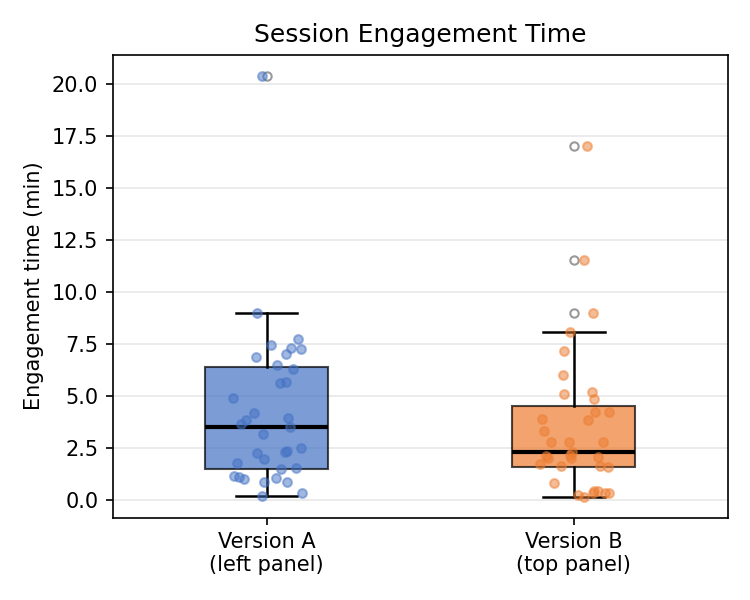
\includegraphics[width=0.5\textwidth]{figures/boxplot_time.png}
\caption{Boxplot of session engagement time (minutes) by version. Version A shows a higher median and several long-session outliers; the difference is not significant.}
\label{fig:box_time}
\end{figure}

\subsection{Secondary Outcomes}

Fisher's exact tests were used for all binary outcomes (Table~\ref{tab:fisher}).

\begin{table}[h]
\centering
\caption{Fisher's exact test results for binary outcomes.}
\label{tab:fisher}
\begin{tabular}{lrrrr}
\hline
\textbf{Outcome} & \textbf{A rate} & \textbf{B rate} & \textbf{OR} & \textbf{$p$-value} \\
\hline
Bounce rate         & 5.7\% (2/35) & 20.0\% (7/35) & 4.13 & 0.151 \\
Export rate         & 5.7\% (2/35) & 2.9\%  (1/35) & 0.49 & 1.000 \\
Workflow completion & 5.7\% (2/35) & 2.9\%  (1/35) & 0.49 & 1.000 \\
\hline
\end{tabular}
\end{table}

None of the secondary outcomes reached statistical significance at $\alpha = 0.05$. The bounce rate odds ratio of 4.13 in favour of more bouncing in Version B is descriptively notable but underpowered given the small counts involved.

\begin{figure}[H]
\centering
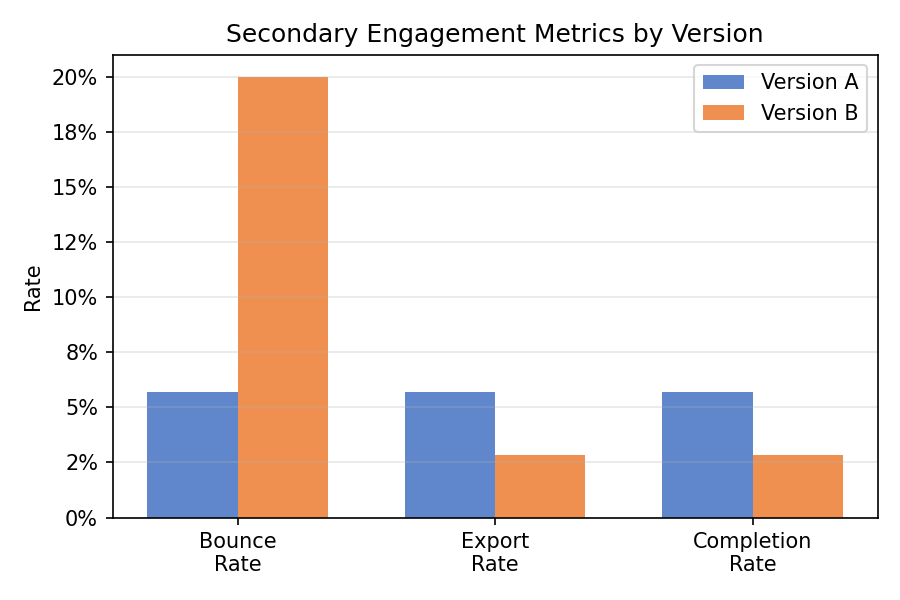
\includegraphics[width=0.60\textwidth]{figures/bar_secondary_metrics.png}
\caption{Secondary engagement metrics by version. Version B has a noticeably higher raw bounce rate; export and completion rates are near-zero in both groups.}
\label{fig:bar_secondary}
\end{figure}

\subsection{Summary of Hypothesis Tests}

All tests fail to reject the null hypothesis $H_0$ at $\alpha = 0.05$. The primary null hypothesis --- that there is no significant difference in sections visited or engagement time between the two layout versions --- is retained.

\section{Interpretation \& Conclusion}

The A/B test found no statistically significant difference between Version A (left-panel upload) and Version B (top-panel upload) on any of the five engagement metrics examined. Both versions produced a median of 3 sections visited per session, suggesting that the majority of users who proceeded past the landing page reached at least the Preprocessing tab in both conditions.

The numerical pattern in the data, however, runs contrary to the treatment hypothesis. Version B users had a lower median engagement time (136.5 s vs.\ 209.6 s) and a higher raw bounce rate (20.0\% vs.\ 5.7\%), though neither difference is statistically significant. Several explanations for this counter-intuitive direction merit consideration.
 
First, the layout manipulation may have been too subtle to overcome motivational factors. Both versions require the identical cognitive step of selecting a dataset before proceeding, meaning the primary barrier to entry, deciding whether to engage with the tool at all, was unchanged. Users' prior domain familiarity and intrinsic motivation to explore likely dominated any effect of control placement.
 
Second, the top-panel layout in Version B may have introduced unfamiliar visual complexity for users accustomed to the conventional sidebar paradigm in Shiny applications. Placing two equal-width control cards horizontally at the top, while relocating the summary metric cards to a vertical left column, departs from the standard convention. Users encountering an unconventional layout may have disengaged faster rather than exploring further, a pattern consistent with research on interface novelty effects.

Third, the higher bounce rate in Version B (20\% vs.\ 5.7\%) may partly reflect link distribution timing. If Version B links were shared later or to less motivated participants, group-level motivational differences could produce apparent layout effects that are in fact selection artifacts.

The very low completion and export rates in both groups (under 6\%) indicate that the six-step workflow is rarely traversed end-to-end under naturalistic, uninstructed conditions, regardless of layout. This may reflect the exploratory nature of the recruitment population: class participants who briefly tested the app without a specific analytical goal.

In conclusion, our experiment provides no evidence that moving the data-loading controls from a sidebar to a top-horizontal layout meaningfully changes how deeply users engage with the application. The directional pattern --- if anything favoring the control condition --- suggests that future work should evaluate whether the top-panel layout introduces unexpected usability friction. A larger, more diverse user base with explicit task instructions would be needed to draw firmer conclusions.

\section{Challenges \& Limitations}

\paragraph{Small sample size and statistical power.}
With $n = 35$ per group, the study is substantially underpowered. A post-hoc power analysis for the Mann-Whitney U test, using the observed rank-biserial $r = -0.135$ for engagement time and $\alpha = 0.05$ (two-sided), yields power below 20\%. This means the experiment would miss a true effect of the observed magnitude more than 80\% of the time. The null results should therefore be interpreted as inconclusive rather than as evidence that the layouts are equivalent.

\paragraph{Non-probability sampling and self-selection.}
Participants were recruited primarily from a single course cohort and through direct link sharing, not random sampling from a target population. Users who chose to interact longer may systematically differ from those who left immediately, introducing selection bias. The between-subjects design mitigates within-subject confounding, but cannot rule out pre-existing group differences.

\paragraph{Ecological validity of GA4 engagement metrics.}
GA4's engagement time is derived from foreground-tab activity and may not accurately reflect genuine cognitive engagement. A user who loads the app and leaves the tab open while attending to other tasks would accumulate engagement time without actually using the product. This measurement artifact could explain the high variance in session duration observed in both groups.

\paragraph{Synthetic data augmentation.}
The dataset combines real user sessions collected via GA4 with simulated sessions generated to reach a sample size of 35 per group (approximately 7 real and 28 synthetic per group; 20\% real, 80\% synthetic). Simulated sessions were drawn to be statistically consistent with the real data distributions, but they reduce the ecological validity of the findings. Any generalisation beyond the observed sample should account for this composition.

\paragraph{Single manipulation; no replication.}
The experiment tests one specific layout change in one application. The finding (or lack thereof) does not generalise to other UI modifications, other Shiny apps, or other user populations. The experiment was run once over a four-week window; replication across different time periods or cohorts would strengthen the conclusions.

\paragraph{Confounding via link distribution.}
Because users self-selected which link to click (rather than being randomly redirected from a single entry point), it is possible that the two groups differed in ways correlated with link distribution (e.g., Version A was shared earlier, reaching more motivated early adopters). URL-parameter or cookie-based randomisation from a single entry point would have provided stronger causal guarantees.

\newpage
\section*{Contributions}

Each member of the team contributed to different aspects of the project.

\begin{itemize}
    \item \textbf{Jason Zhao (zz3390)}  prepared the A/B test experiment and split the code, deploying both versions with event tracking through Google Analytics 4.

    \item \textbf{Sebastian Hoornweg (smh2289)} handled the organization and statistical processing of user data collected from the experiment, including the synthetic data generation and validation procedure.

    \item \textbf{Yuhan Guo (yg2695)} conducted the data analysis part and was primarily responsible for writing the report.

    \item \textbf{Omari Motta (osm2116)} performed consistency checks across all sections and contributed to improving the interpretation and limitations discussion.
\end{itemize}

\end{document}
